\chapter{Implementace}

\section{Implementace API}
Implementace původně probíhala ve frameworku FastAPI \sectionref{sec:api_technologies:fast} ale po zjištění složitosti ORM při použití Python knihovny SQL Alchemy bylo doporučeno jedním z řešitelů (P. Mikula)
použít raději Javu a její Spring boot framework, za použití knihoven jako je JPA , Lombok, Jackson a jiných. Tato změna nebyla obtížná, jelikož vývoj byl teprve ve velice ranní fázi vývoje. Taktéž Spring Boot byl jeden z kandidátů.

Nyní budou popsány nejdůležitější knihovny Frameworku Spring Boot, které byly použity při implementaci API.


\subsection{Spring Boot knihovny}\label{sec:impl:spring} 
% TODO nějaký lepší název nebo něco

Tyto knihovny jsou základní stavební kámen jak pro samotné koncové body tak pro \gls{orm}. Na obrázku \figureref{fig:JPA} máme vizuální schéma jak magie ORM ve Spring Bootu funguje

\begin{figure}[ht!]
    \centering
    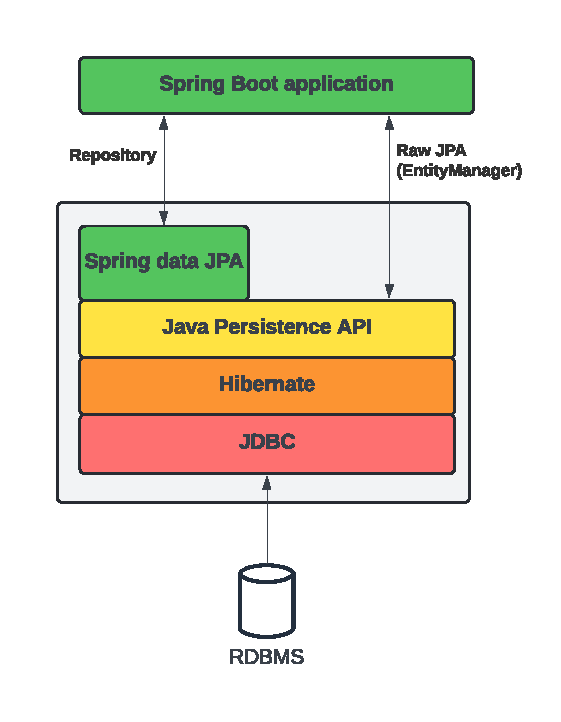
\includegraphics[width=0.5\textwidth]{figures/impl/API Implementation - JPA.pdf}
    \caption{Struktura Spring Boot Data JPA aplikace}
    \label{fig:JPA}
\end{figure}

\subsubsection*{Spring Data JPA}
Neboli Java Persistence API je jedna ze součástí Spring Data Family, která umožnuje jednoduché implementování \textbf{repozitářů} založených na JPA. Signifikantně zjednodušuje implementaci datové vrstvy aplikace. Umožňuje používat základní SQL požadavky a ORM bez námahy případně si vytvořit své vlastní požadavky. V ukázce \coderef{code:JPA_repo} je vidět implementace repositáře pro entitu \textit{Enemy}. Zde jsou již naimplementované základní metody jako \textit{save}, \textit{findAll}, a je zde navíc metoda \textit{findAllByLocationId} s vlastním SQL dotazem.

\begin{listing}[ht!]
    \inputminted[]{Java}{resources/code/impl/EnemyRepo.java}
    \caption{Ukázka JPA repositáře}
    \label{code:JPA_repo}
\end{listing}

\subsubsection*{JPA}
Spring data JPA používá několik dalších knihoven a dalo by se říci že to je jakýsi zprostředkovatel nad \textbf{JPA}. JPA je zprostředkovatel objektově relačního mapování (\gls{orm}), což usnadnuje práci s ukládáním objektů do databáze a naopak.

Základním objektem v JPA je \textit{Entita}. Ta reprezentuje objekt v databázi který je poté namapován na jednotlivé vlastnosti třídy \coderef{code:jpa_entity}.
Třídu označíme jako entitu pomocí anotace \textit{@Entity} a poté pomocí \texttt{@Table} můžeme upřesnit jméno tabulky, schéma databáze a jiné.Za pomoci anotace \textit{@Id} označíme primární klíč a nebo pomocí \texttt{@EmbeddedId} označíme složený primární klíč. Atributy třídy označíme pomocí \texttt{@Column} kdy ve výchozím stavu atribut může nabývat prázdné hodnoty a sloupec v databázi se jmenuje stejně jako atribut. Relace se mapují pomocí jedné z anotací \texttt{@OneToOne}, \texttt{@OneToMany}, \texttt{@ManyToOne}, \texttt{@ManyToMany} podle toho jakou relaci potřebujeme. V této implementaci probíhal nejdříve návrh databáze, takže jsme používali pouze 1:n relace abychom se vyhnuli cyklickým závislostem protože m:n spojovací tabulky již byly v databázi.

\subsubsection*{Hibernate}\label{sec:impl:hibernate}
Jedna z konkrétních implementací JPA je Hibernate. Udržuje si za pomocí výše zmíněných anotací nebo XML \sectionref{sec:formats:xml} schématu schéma databáze a stav objektů, tedy udržuje data perzistentní. Díky schématu databáze Hibernate ví jak se mají transformovat data z databázových tabulek do objektů a naopak. \cite[]{enwiki:1217225259}

\subsubsection*{JDBC}\label{sec:impl:jdbc}
Neboli Java Database Connectivity je API pro přístup k databázi. Poskytuje metody pro dotazování se na na databázi pomocí \gls{sql}, a umožňuje zpracovávat výsledky dotazů.

\begin{listing}[ht!]
    \inputminted[]{Java}{resources/code/impl/EnemyDTO.java}
    \caption{Příklad entity v JPA}
    \label{code:jpa_entity}
\end{listing}


\subsection{Ostatní použité knihovny} %%TODO reformat nadpis aaaaaa
V této kapitole budou popsány knihovny, které nejsou součástí Spring Bootu, ale byly použity ve větší míře při implementaci API.

\subsubsection*{Lombok}\label{sec:impl:lombok}
Lombok je knihovna, která automaticky za pomocí anotací generuje základní repetetivní kódy jako jsou gettery a settery, konstruktory a jiné. Nebál bych se říci, že když jednou vyzkoušíte Lombok, tak se stane pro vás nedílnou součástí Javy.

Jako první věc jsou anotace \texttt{@Getter} a \texttt{@Setter} které automaticky vygenerují \textbf{gettery} nebo \textbf{settery} s příslušnými modifikátory přístupu pro daný atribut \coderef{code:lombok:getters}. Ovšem tato anotace lze použít i nad celou třídou a automaticky vygeneruje kód pro všechny atributy. Vygenerované gettery a settery vypadají takto: \ref{code:lombok:getters:generated}
\begin{listing}[H]
    \begin{minted}[fontsize=\footnotesize]{Java}
        public class GetterSetterExample {
            @Getter private int age = 10;
            @Setter(AccessLevel.PROTECTED) private String name;
        }
     \end{minted}
    \caption{Použití anotací \texttt{@Getter} a \texttt{@Setter}}
    \label{code:lombok:getters}
\end{listing}

\begin{listing}[H]
    \begin{minted}[fontsize=\footnotesize]{Java}
        public class GetterSetterExample {
            private int age = 10;
            private String name;
            public int getAge() {
                return this.age;
            }
            protected void setName(String name) {
                this.name = name;
            }
        }
     \end{minted}
    \caption{vygenerovaný kód za pomocí \texttt{@Getter} a \texttt{@Setter}}
    \label{code:lombok:getters:generated}
\end{listing}

Další důležité anotace jsou konstruktorové anotace. \texttt{@NoArgsConstructor} vygeneruje prázdný konstruktor, \texttt{@AllArgsConstructor} vygeneruje konstruktor se všemi atributy \coderef{code:lombok:constructor} a jako poslední konstruktor \texttt{@RequiredArgsConstructor} vygeneruje konstruktor s všemi atributy označenými jako \texttt{@NonNull}. Tato anotace se dává nad třídu. \cite{lombok:constructor} 

\begin{listing}[H]
    \begin{minted}[fontsize=\footnotesize]{Java}

        public class ConstrExample {
            private int age;
            private String name;

            ConstrExample(int age, String name) {
                this.age = age;
                this.name = name;
            }
        }
    
    \end{minted}
    \caption{Příklad kódu vygenerovaného pomocí \texttt{@AllArgsConstructor}}
    \label{code:lombok:constructor}
\end{listing}


Práce se může ještě více zjednodušit za pomocí anotace \texttt{@Data} která vygeneruje výše zmíněné \texttt{@Getter, @Setter, @RequiredArgsConstructor} a navíc \texttt{@ToString} a \texttt{@EqualsAndHashCode} \cite{lombok:data}.
Anotace \texttt{@ToString} vygeneruje metodu \texttt{toString()} která objekt převede na textový řetězec a za pomocí různých parametrů můžeme upravovat jaké atributy se budou vypisovat a jak. Další anotace co \texttt{@Data} obsahuje je \texttt{@EqualsAndHashCode} která vygeneruje metody pro porovnávání objektů.


Za zmínku ještě stojí anotace \texttt{@Builder} která vygeneruje interní třídu podle návrhového vzoru Builder\cite{refactoringGuru:builder} podle která slouží k vytváření objektů. \cite{lombok:builder}

\subsubsection*{Jackson}\label{sec:impl:jackson}
Tato knihovna slouží pro serializaci objektů do formátu JSON \chapterref{sec:formats:json} a naopak. Za pomocí této knihovny bylo možné specifikovat jak se budou jednotlivé objekty či atributy serializovat. Jako je například ignorování některých atributů a nebo vlastní serializace.

\subsubsection*{Swagger}\label{sec:impl:swagger}
Swagger je open-source dokumentační nástroj, který je již spolu se Spring bootem, pro RESTful API, který umožňuje vývoj API skrz celý jeho životní cyklus od návrhu přes dokumentaci a testování po nasazení. Využívá specifikaci OpenAPI, pomocí které dokáže generovat dokumentaci, interakci,  testy a další. \cite{swagger:about}
Tohoto nástroje jsme hojně využívali zvlášť pro interakci s koncovými body pro testování.

Ve Spring Bootu se velice jednoduše používá, stačí přidat závislosti do \texttt{pom.xml} a přidat Springdoc Swagger konfiguraci do hlavního konfiguračního souboru.

\subsection{Serializace}\label{sec:impl:serialization}
\sectionref{sec:formats:deserialization} 
Byla vytvořena vlastní třída pro serializaci relačních objektů pomocí vlastní třídy 
%\coderef{code:lazyFieldsSerializer} TODO
na serializování mapovaných objektů. Přepsaná metoda \texttt{serialize} zde zkontroluje zda je serializovaný objekt instancí proxy a pokud ano tak zda je objekt nainicializován. To za nás řeší metoda \texttt{Hibernate.isInitialized} 
%\coderef{code:lazyFieldsSerializer}[, řádek 56]. TODO
Pokud tedy objekt je nainicializován tak se serializuje a dále na jeho atributech se opět volá metoda \texttt{serialize}. Pokud není nainicializován a není to kolekce tak se serializuje pouze jeho id aniž by se objekt nainicializoval 
%\coderef{code:lazyFieldsSerializer}[, řádek 60]. TODO
A pokud to je kolekce tak se musí jednat o m:n tabulku a serializují se tedy všechny atributy kromě relací. 
%\coderef{code:lazyFieldsSerializer}[, funkce \texttt{writeFieldsWithoutLazy() }]. TODO


\subsection{Lazy load}\label{sec:impl:lazyload}
Pro tento účel musela být vytvořena metoda pro postupnou inicializaci. Pro rekurzivní načítání relačních objektů byla vytvořena statická metoda \texttt{.hibernateInitializeAll()}, která přijme objekt a rekurzivně načte všechny jeho relace. 
% nějaký ref
Tato funkce za pomocí \texttt{Hibernate.initilize()} nejdříve nainicializuje vstupní objekt a poté rekurzivně prochází všechny jeho atributy. Ovšem přeskakuje atributy které nemají jednu z relačních anotací. Funkce má taktéž podporu filtru pro samotný lazy load, kdy když jméno atributu se shoduje s jakýmkoli slovem ve filtru, atribut se přeskočí v inicializování.


\subsection{Koncové body}\label{sec:impl:endpoints}
Hlavním výstupem této práce je seznam koncových bodů jak pro administrativní část tak pro hraní hry. Jednotlivé přístupové body jsou rozděleny do tzv. kontrolérů. Jako příklad zde je kontrolér pro entitu \textit{Enemy} \coderef{code:characterController}. 

% \begin{figure}[H] %TODO graf endpointu
%     \centering
%     \includegraphics[width=0.7\textwidth]{figure}
%     \caption{caption}
%     \label{fig:label}
% \end{figure}

Anotací \texttt{@RestController} určíme že tato třída bude obsahovat koncové body. Dále pomocí anotace \texttt{@RequestMapping} určíme cestu pod kterou budou všechny koncové body v této třídě dostupné. A naposledy pomocí jednotlivých mapping anotací (\texttt{@GetMapping, @PutMapping @PostMapping @DeleteMapping}) určujeme na jakou HTTP metodu má funkce reagovat. 

Při mapování můžeme určovat jak URI vzory pomocí regex výrazů (např \texttt{"/resources/*.png"}) tak i proměnné v URI (např \texttt{"/resources/{id}"}). Ten používáme třeba zde \coderef{code:characterController}[, řádek 9] pro získání jedné entity \textit{Enemy}. S tím se pojí anotace \texttt{@PathVariable} která určuje, že vstupní parametr id bude brán z URI a bude se jednat o datový typ \texttt{int}. 

Jako další tzv. \textit{query} parametry můžeme získat za pomocí anotace \texttt{@RequestParam}, kde se může předem určit zda je parametr povinný nebo jakou bude mít výchozí hodnotu. \coderef{code:characterController}[, řádek 12]. ve výsledné URI požadavek pro získání entity s identifikátorem 1 a s načteným inventářem bude vypadat takto \texttt{GET /characters/1?include\=inventory\&lazy=true}. Tento požadavek vrátí postavu hráče s namapovaným inventářem a s ostatními atributy. Atributy \textit{clazz} a \textit{race} TODO ref na db schema
 budou vypsané pouze jako id a nebudou nainicializované. 

Pro metody post byla ještě použita anotace \texttt{@RequestBody}, pomocí které můžeme vzít data z těla požadavku. V našem případě jsme požadovali JSON objekt, který se hned mapoval na objekt třídy.

\begin{listing}[ht!]
    \inputminted[]{Java}{resources/code/impl/CharacterController.java}
    \caption{Kontrolér pro entitu \textit{Character}}
    \label{code:characterController}
\end{listing}


\section{Testování}\label{sec:testing}
Testování probíhalo za pomocí dobrovolníků kteří si zkusili zahrát hru a nebo zkoušeli. Díky dokumentačnímu rozhraní Swagger \sectionref{sec:impl:swagger}
bylo možné aby dobrovolníci přímo koncové body v API pohodlně testovali.



\section{Problémy při vývoji}
Během vývoje se vyskytlo několik problémů, které se musely vyřešit. Nyní se zaměříme na ty nejzávažnější.
\subsection{Serializace} %%TODO tohle ref nefunguje idk why
Když byly atributy označeny, že mají být načteny z databáze až při přístupu k danému atributu, tak pořád byl problém při serializaci, protože knihovna Jackson samozřejmě k těmto atributům přistupovala a tím pádem tyto atributy byly načteny z databáze i když se v kódu s nimi nepracovalo a serializovala je. Tento problém byl vyřešen pomocí vlastní třídy 
%\coderef{code:lazyFieldsSerializer} 
na serializování namapovaných objektů. \sectionref{sec:impl:serialization}

\subsection{Lazy load}
Bohužel knihovna Hibernate nemá metodu pro rekurzivní načtení jeho relací, tohle v souvislosti s vlastní serializací byl problém když se měl serializovat objekt se všemi jeho relacemi. Hibernate podporuje jen načtení objektu který je instancí \texttt{HibernateProxy}. Tento problém byl vyřešen pomocí statické funkce \texttt{hibernateInitializeAll()}. \sectionref{sec:impl:lazyload}

\subsection{Příliš velká databáze}
%TODO idk jestli všechno zz toho tu nechat nebo to trošku prostříhat
Při návrhu databáze nebyl brán ohled na možnou časovou náročnost. Databáze se navrhovala jako funkční celek připravený do produkce i s ohledem na případné rozšíření. To vyústilo v to že jednotlivé případné úkony jako je \gls{orm} či CRUD operace nad jednotlivými entitami byly velice zdlouhavé a zabíraly většinu času vývoje. S tímto se pojil o to složitější management změn u koncových bodů. Taktéž z tohoto důvodu se v implementaci vynechaly entity \textit{summon} a \textit{item}.
